\documentclass{beamer}

% Theme selection (e.g., Madrid, or default)
\usetheme{Madrid} % A common, clean theme

% Color theme (optional)
% \usecolortheme{default}

% Font theme (optional)
% \usefonttheme{default}

\usepackage{graphicx} % For including images
\usepackage{hyperref} % For clickable links (optional)
\usepackage{amsmath}
\usepackage{amsfonts}
\usepackage{amssymb}

% Title page information
\title{Leveraging AI/ML for Proactive Anomaly Detection and Self-Healing in Software-Defined Networks (SDN)}
\author{Xiangyi Li}
\institute{Student ID: 017415996 \\ CS 258 - Computer Communication Systems}
\date{May 2025}

\begin{document}

% Title Page
\begin{frame}
  \titlepage
\end{frame}

% Table of Contents (optional, can be added if desired)
% \begin{frame}{Outline}
%   \tableofcontents
% \end{frame}

% --- Section 1: Introduction ---
\section{Introduction}

\begin{frame}{Introduction: The Evolving Network Landscape \& Problem}
  \frametitle{The Evolving Network Landscape \& Problem}
  \begin{itemize}
    \item \textbf{The Evolving Network Landscape:}
    \begin{itemize}
        \item Modern communication networks are experiencing unprecedented growth in scale, complexity, and the diversity of services they support. From massive IoT deployments to cloud computing and the burgeoning demands of 5G/6G, networks are more critical and intricate than ever.
        \item Software-Defined Networking (SDN) has emerged as a paradigm shift, offering centralized control and programmability, which brings agility and innovation to network management. However, this centralization and programmability also introduce new challenges and vulnerabilities.
    \end{itemize}
    \item \textbf{Problem Statement:}
    \begin{itemize}
        \item Despite their advantages, SDNs are susceptible to a range of sophisticated cyber threats, including Distributed Denial of Service (DDoS) attacks that can overwhelm the control plane or data plane resources. As highlighted by Al-Janabi \& Al-Shourbaji (2024) in their survey, DDoS attacks remain a significant concern in SDN environments, capable of causing severe service disruptions.
        \item Beyond external attacks, SDNs can also suffer from internal system faults, misconfigurations, and unexpected anomalies that degrade performance or lead to outages.
        \item Traditional security measures and manual intervention often fall short in providing the rapid, adaptive, and scalable responses needed to counter these dynamic threats and ensure network resilience.
    \end{itemize}
  \end{itemize}
\end{frame}

\begin{frame}[shrink]{Introduction: Motivation, AI/ML Promise \& Roadmap}
  \frametitle{Motivation, AI/ML Promise \& Roadmap}
  \begin{itemize}
    \item \textbf{Motivation:}
    \begin{itemize}
        \item The increasing reliance on robust and secure network infrastructures for critical societal functions—ranging from healthcare and finance to smart cities and autonomous systems—necessitates a move towards more intelligent and autonomous network operations.
        \item There is a compelling need to enhance network security beyond reactive measures, moving towards proactive threat detection and automated remediation to maintain operational continuity and data integrity.
    \end{itemize}
    \item \textbf{The Promise of AI/ML:}
    \begin{itemize}
        \item Artificial Intelligence (AI) and Machine Learning (ML) offer powerful tools to address these complex challenges. By learning from vast amounts of network data, AI/ML algorithms can identify subtle patterns indicative of anomalies, predict potential threats, and orchestrate intelligent responses.
        \item As Edozie et al. (2025) discuss in their review of AI advances in anomaly detection for telecom networks, AI, particularly deep learning, is transformative in handling the dynamism and scale of modern network data, enabling more effective and proactive security measures.
    \end{itemize}
    \item \textbf{Presentation Objectives \& Roadmap:}
    \begin{itemize}
        \item \textbf{Objective:} This presentation will explore how AI/ML techniques can be leveraged to build proactive anomaly detection and self-healing capabilities within SDN environments.
        \item \textbf{Roadmap:}
        \begin{enumerate}
            \item Background on SDN: Core concepts and vulnerabilities.
            \item AI/ML for Anomaly Detection in SDN: Techniques and applications.
            \item AI/ML for Self-Healing in SDN: Mechanisms and approaches.
            \item A Proposed Integrated AI/ML Framework.
            \item Key Challenges and Future Research Directions.
            \item Conclusion.
        \end{enumerate}
    \end{itemize}
  \end{itemize}
\end{frame}

% --- Section 2: Background on SDN ---
\section{Background on SDN}

\begin{frame}{Background: Software-Defined Networking (SDN) - Core Concepts}
  \frametitle{Core Concepts of SDN}
  \begin{itemize}
    \item \textbf{Core Concepts of SDN:}
    \begin{itemize}
        \item \textbf{Decoupling of Control and Data Planes:} The control plane (decides how traffic is handled) is separated from the data plane (forwards traffic).
        \item \textbf{Centralized Control:} Network intelligence is logically centralized in an SDN controller, providing a global network view.
        \item \textbf{Programmability:} Network behavior can be programmed via open interfaces (e.g., OpenFlow).
    \end{itemize}
    \item \textbf{Key Architecture Layers:}
    \begin{itemize}
        \item \textbf{Infrastructure Layer (Data Plane):} Network devices (switches, routers) that forward packets.
        \item \textbf{Control Layer:} SDN controller(s) making decisions and managing resources.
        \item \textbf{Application Layer:} Network applications leveraging controller capabilities.
    \end{itemize}
  \end{itemize}
  \begin{figure}
    \centering
    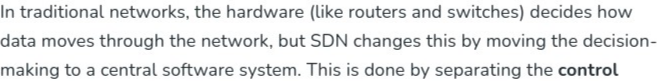
\includegraphics[width=0.7\textwidth]{figures/geeksforgeeks_sdn_architecture.png}
    \caption{SDN Architecture. Source: geeksforgeeks.org}
  \end{figure}
\end{frame}

\begin{frame}{Background: SDN Benefits \& Inherent Vulnerabilities}
  \frametitle{SDN Benefits \& Inherent Vulnerabilities}
  \begin{itemize}
    \item \textbf{Benefits of SDN:} Agility, Centralized Management, Innovation, Improved Operational Efficiency.
    \item \textbf{Inherent Vulnerabilities in SDN:}
    \begin{itemize}
        \item \textbf{Control Plane Saturation:} Controller as a bottleneck (Rathore et al., 2024).
        \item \textbf{Data Plane Attacks:} Exhausting switch resources.
        \item \textbf{Compromised Controller:} Entire network subversion.
        \item \textbf{Interface Security:} Southbound/Northbound API vulnerabilities.
        \item \textbf{New Attack Surfaces:} Due to programmability and centralization.
    \end{itemize}
  \end{itemize}
  \begin{figure}
    \centering
    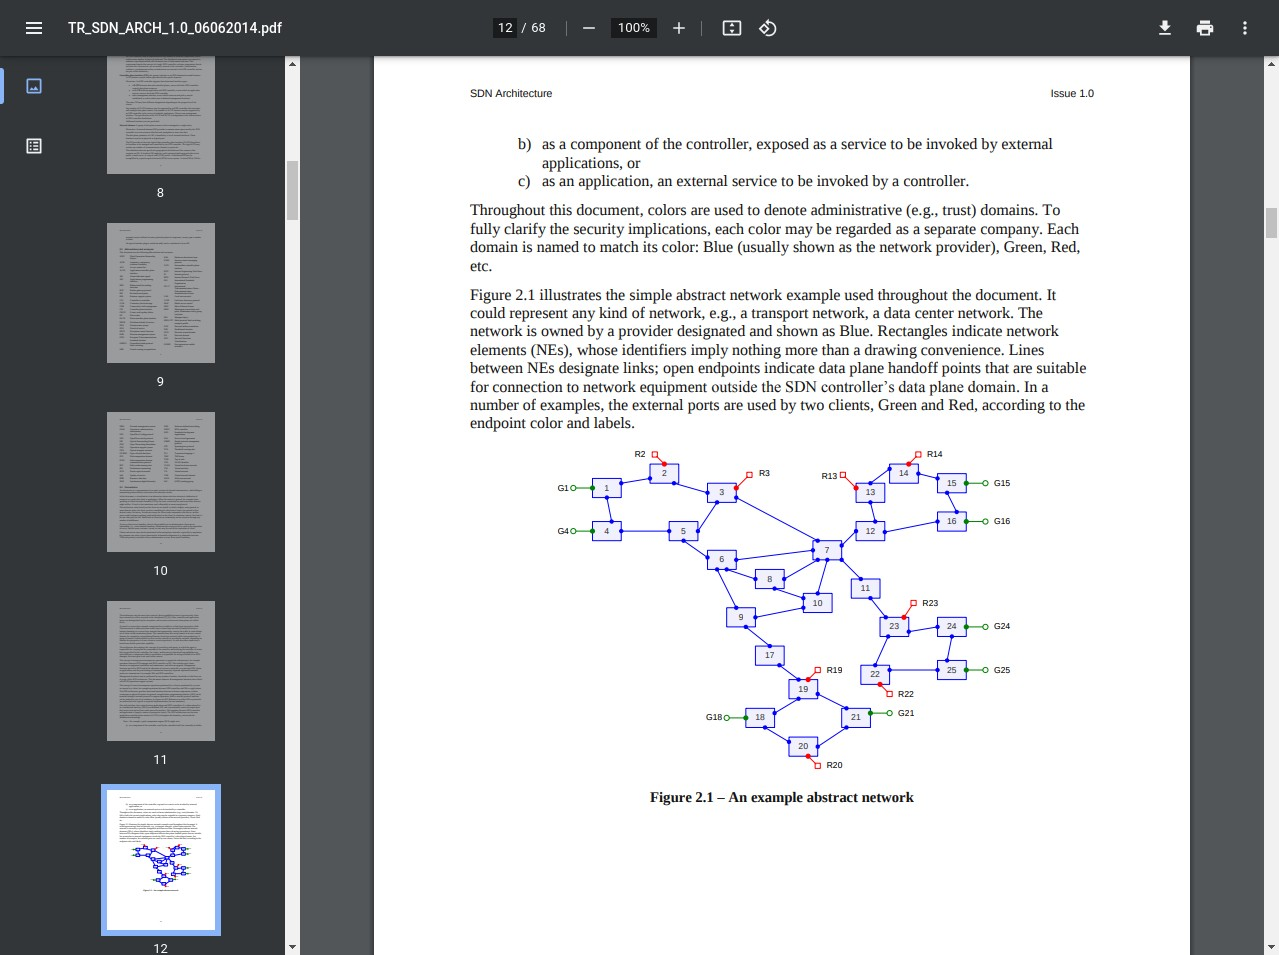
\includegraphics[width=0.6\textwidth]{figures/onf_sdn_figure_2_1_abstract_network.png}
    \caption{Example Abstract Network. Source: ONF TR-502, SDN Architecture Issue 1.0}
  \end{figure}
\end{frame}

% --- Section 3: AI/ML for Anomaly Detection in SDN ---
\section{AI/ML for Anomaly Detection in SDN}

\begin{frame}{AI/ML for Anomaly Detection in SDN: Why AI/ML?}
  \frametitle{Why AI/ML for Anomaly Detection?}
   \begin{itemize}
    \item \textbf{Learning Complex Patterns:} Identify novel/zero-day exploits (Al-Janabi \& Al-Shourbaji, 2024).
    \item \textbf{Adaptability:} Continuously train and update for new threats (Edozie et al., 2025).
    \item \textbf{Handling Large Data Volumes:} Process vast SDN telemetry data.
    \item \textbf{Automation:} Reduce manual analysis, enable faster responses.
    \item \textbf{Improved Accuracy:} Aim to reduce false positives (Latif et al., 2022).
  \end{itemize}
\end{frame}

\begin{frame}{AI/ML for Anomaly Detection in SDN: Key Techniques}
  \frametitle{Key AI/ML Techniques for Anomaly Detection}
  \begin{itemize}
    \item \textbf{Machine Learning Classifiers:} (SVM, Decision Trees, Random Forest) - Latif et al. (2022).
    \item \textbf{Deep Learning Models:} (DNN, RNN, LSTM, Autoencoders) - Agnihotri et al. (2025).
    \item \textbf{Graph Neural Networks (GNNs):} Leverage network topology (GraphSAGE) - Rathore et al. (2024).
    \item \textbf{Generative Adversarial Networks (GANs):} Detect novel anomalies - Kim et al. (2024).
    \item \textbf{Data Sources \& Feature Engineering:} Critical for effective detection.
  \end{itemize}
  \begin{figure}
    \centering
    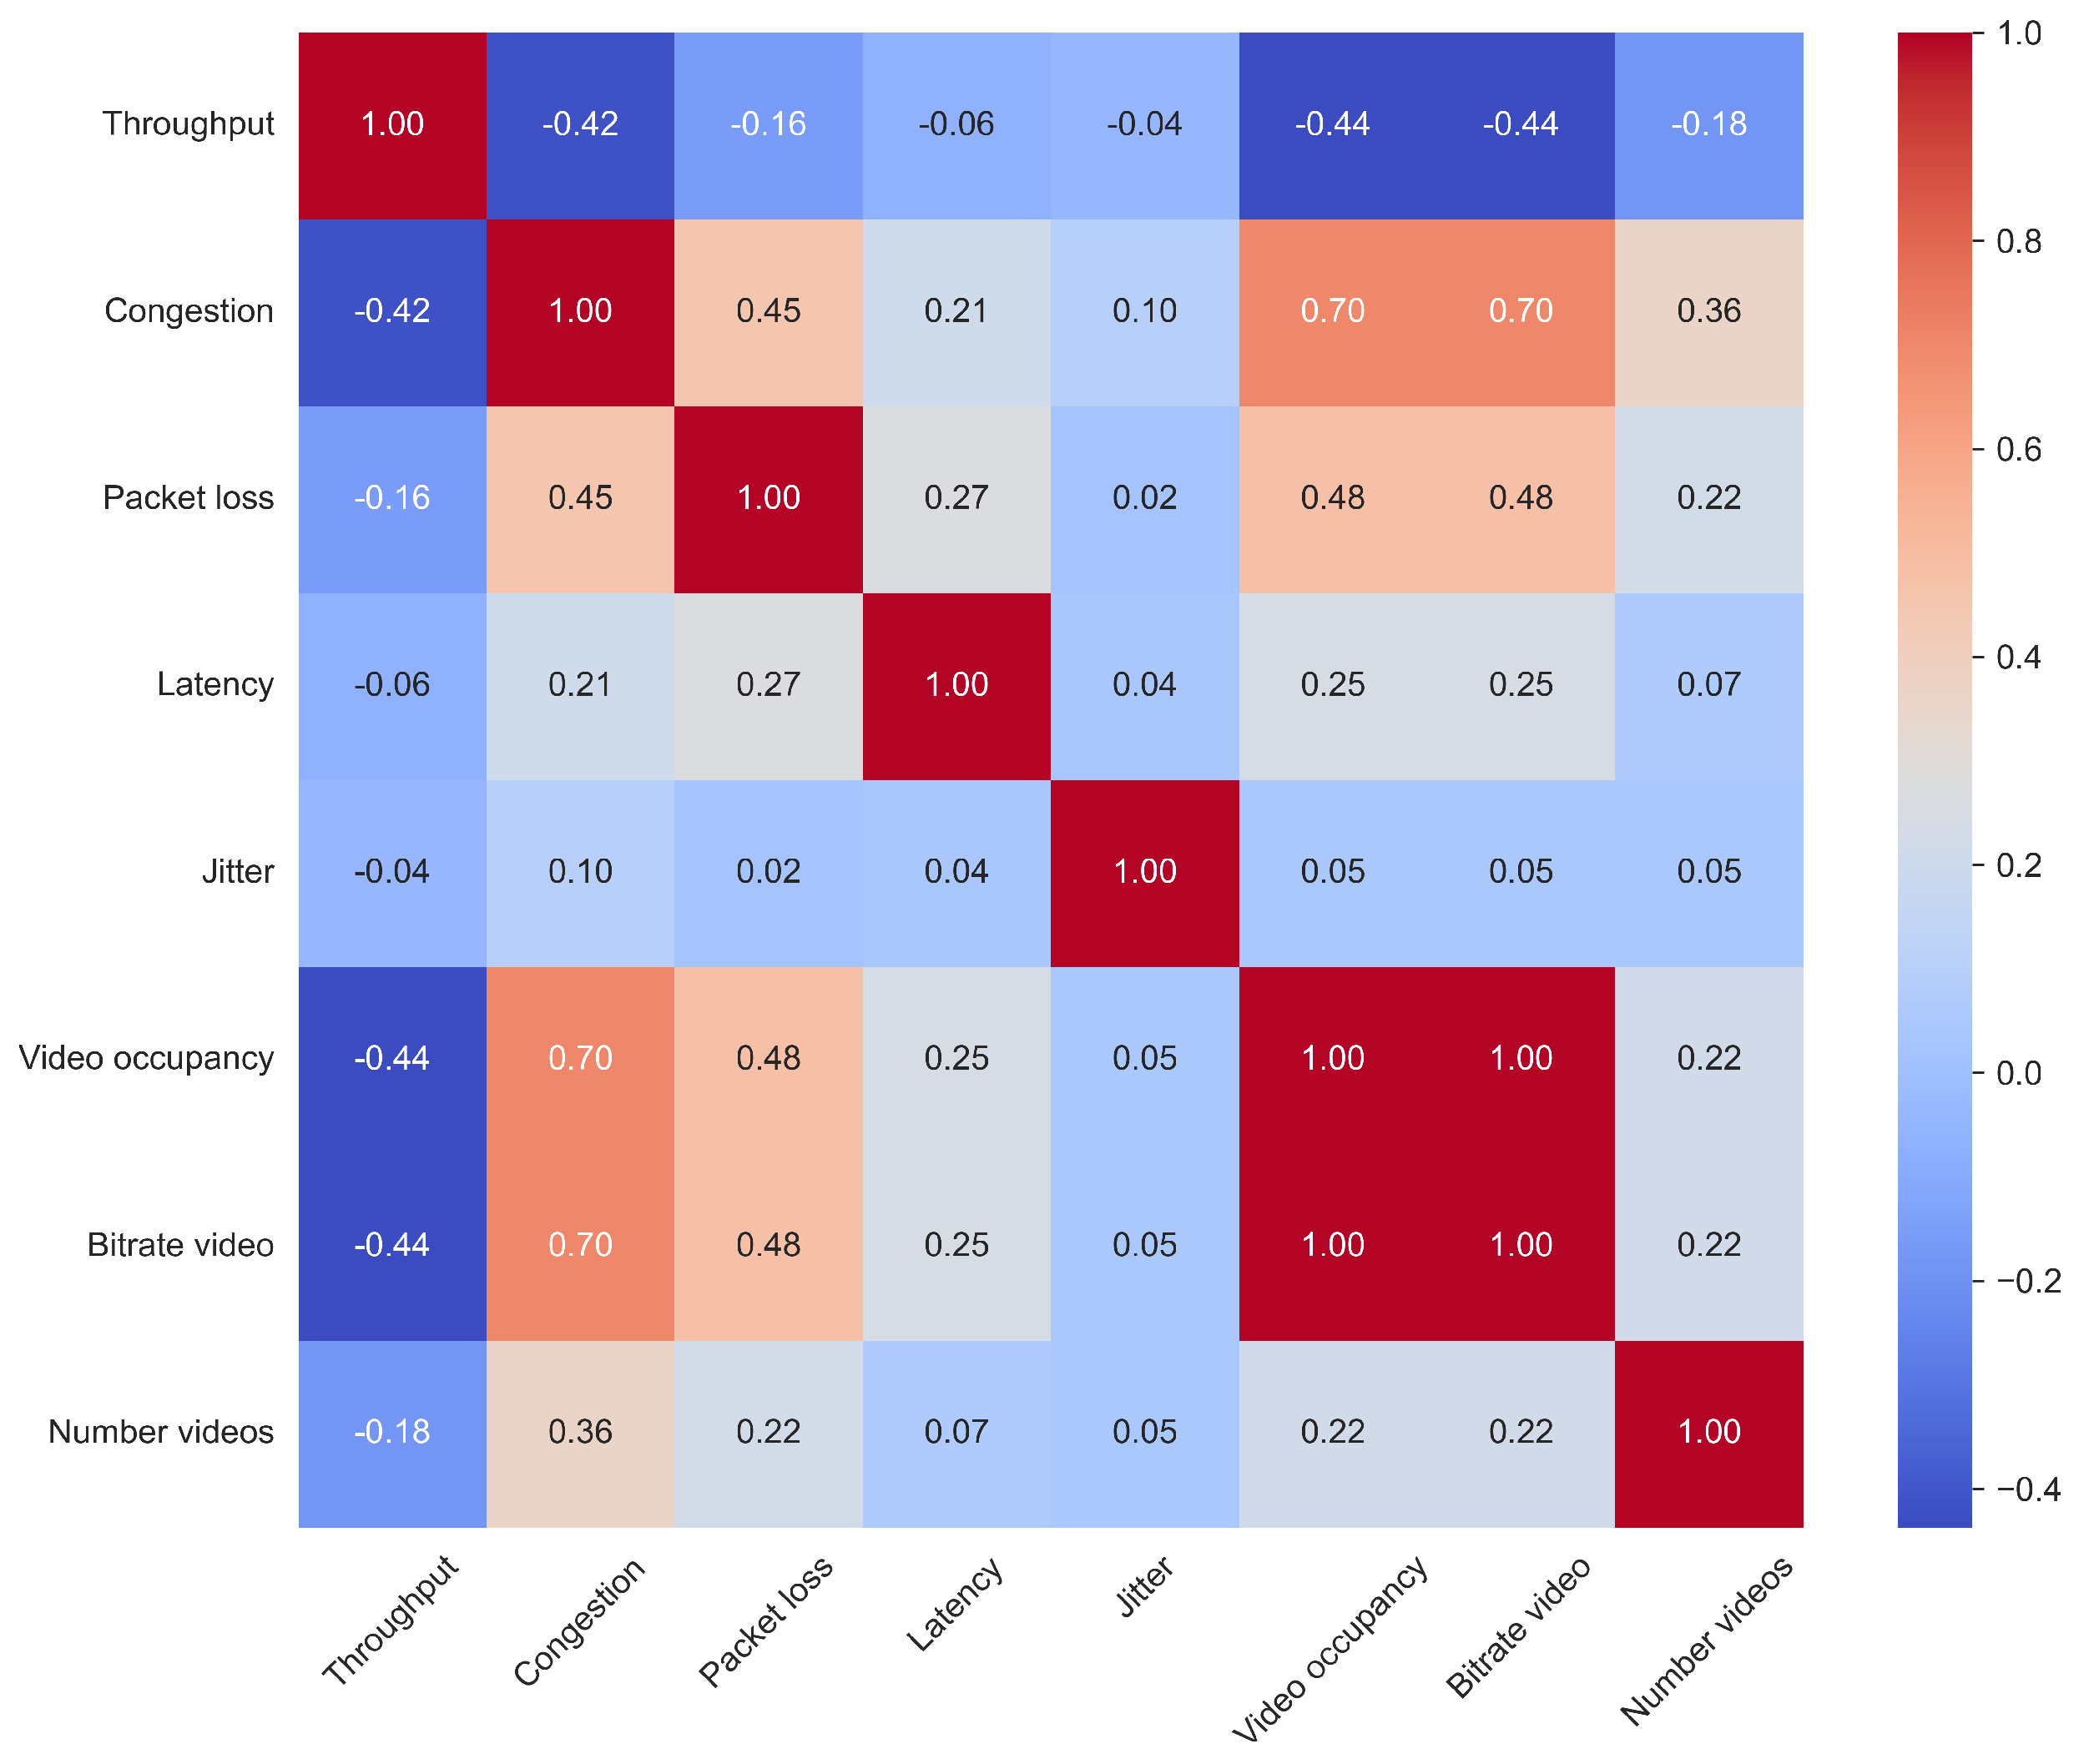
\includegraphics[width=0.6\textwidth]{figures/mdpi_correlation_matrix_ai_ml.png}
    \caption{Correlation Matrix for Network Anomaly Features. Source: MDPI (doi:10.3390/ai5040143)}
  \end{figure}
\end{frame}

% --- Section 4: AI/ML for Self-Healing in SDN ---
\section{AI/ML for Self-Healing in SDN}

\begin{frame}{AI/ML for Self-Healing in SDN: Concepts and Mechanisms}
  \frametitle{Concepts and Mechanisms}
  \begin{itemize}
    \item \textbf{Concept of Self-Healing Networks:} Automated fault detection, diagnosis, and recovery.
    \item \textbf{Role of AI/ML:} Enabling intelligent decision-making for remediation, predictive maintenance (Costa et al., 2023).
    \item \textbf{Key Mechanisms:} Automated fault localization, intelligent traffic re-routing, dynamic resource re-allocation, automated policy updates.
    \item \textbf{Reinforcement Learning:} For learning optimal recovery strategies.
  \end{itemize}
  \begin{figure}
    \centering
    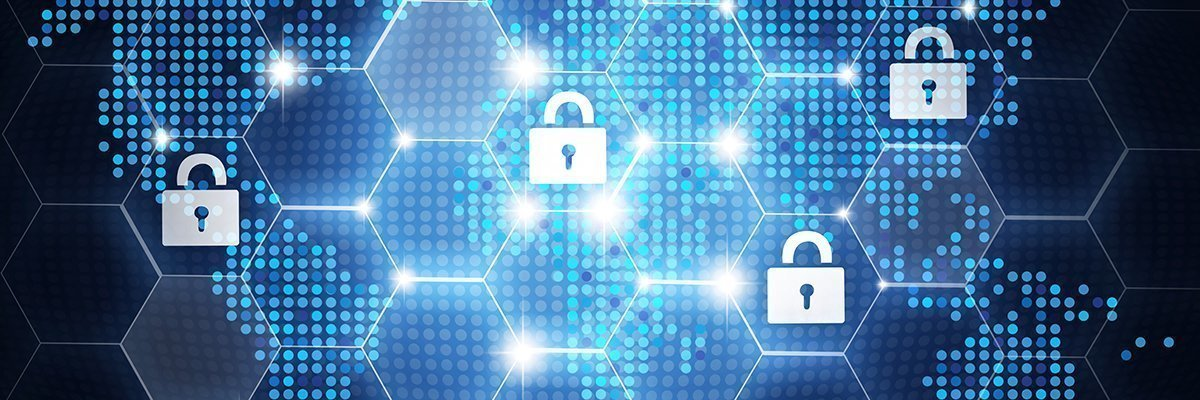
\includegraphics[width=0.6\textwidth]{figures/computerweekly_self_healing_network_concept.jpeg}
    \caption{Self-Healing Network Concept. Source: computerweekly.com}
  \end{figure}
\end{frame}

% --- Section 5: Proposed Integrated AI/ML Framework ---
\section{Proposed Integrated AI/ML Framework}

\begin{frame}{Proposed Integrated AI/ML Framework: Architecture}
  \frametitle{Architecture and Integration}
  \begin{itemize}
    \item \textbf{High-Level Architecture:}
    \begin{itemize}
        \item Data Ingestion \& Preprocessing Module
        \item AI-Powered Anomaly Detection Engine
        \item AI-Driven Decision Support \& Self-Healing Orchestrator
        \item Feedback \& Continuous Learning Module
    \end{itemize}
    \item \textbf{Incorporating New References:} Insights from the 10+ papers strengthen choices for algorithms (e.g., GNNs for detection, RL for orchestration) and architectural considerations.
  \end{itemize}
\end{frame}

% --- Section 6: Key Challenges and Future Directions ---
\section{Key Challenges and Future Directions}

\begin{frame}{Key Challenges and Future Directions}
  \frametitle{Challenges and Future Work}
  \begin{itemize}
    \item \textbf{Data-related:} Quality, quantity, labeling, privacy (Alenezi et al., 2024).
    \item \textbf{Model-related:} Scalability, real-time performance, interpretability (XAI), robustness (Singh \& Rana, 2025).
    \item \textbf{Deployment-related:} Integration, standardization.
    \item \textbf{Security of AI Models:} Protecting AI components (Elsayed et al., 2025).
    \item \textbf{Future Research:} XAI in SDN security, federated learning, proactive threat hunting.
  \end{itemize}
\end{frame}

% --- Section 7: Conclusion ---
\section{Conclusion}

\begin{frame}{Conclusion: Summary and Path Forward}
  \frametitle{Summary and Path Forward}
  \begin{itemize}
    \item \textbf{Summary:} AI/ML holds immense potential for enhancing SDN security and resilience through proactive anomaly detection and self-healing.
    \item \textbf{Importance:} Critical for future networks (5G/6G) and complex communication systems.
    \item \textbf{Path Forward:} Continued research is vital to overcome challenges related to data, model performance, deployment, and the security of AI itself.
  \end{itemize}
\end{frame}

% --- Section 8: References ---
\section{References}

\begin{frame}[allowframebreaks]{References}
  \frametitle{References}
  % Using itemize for now, can switch to BibTeX later if needed
  \begin{itemize}
    \item Al-Janabi, S., \& Al-Shourbaji, I. (2024). Machine Learning and Deep Learning Techniques for Distributed Denial of Service Anomaly Detection in Software Defined Networks—Current Research Solutions. \textit{IEEE Access}.
    \item Rathore, S., Sahoo, G., \& Sahoo, B. (2024). Software defined network and graph neural network-based anomaly detection scheme for high speed networks. \textit{Alexandria Engineering Journal}.
    \item Latif, Z., Umer, Q., Lee, C., et al. (2022). A Machine Learning-Based Anomaly Prediction Service for Software-Defined Networks. \textit{Sensors}.
    \item Edozie, E., Shuaibu, A.N., Sadiq, B.O., et al. (2025). Artificial intelligence advances in anomaly detection for telecom networks. \textit{Artificial Intelligence Review}.
    \item Agnihotri, D., Verma, K., \& Tripathi, R. (2025). Improved network anomaly detection system using optimized deep belief network and feature fusion. \textit{Expert Systems with Applications}.
    \item Kim, J., Kim, J., Kim, H., \& Kim, H. (2024). Generative Adversarial Network Models for Anomaly Detection in Software-Defined Networking. \textit{Journal of Network and Systems Management}.
    \item Costa, E. F., Piamrat, K., \& Nogueira, M. (2023). AI-driven self-healing in software-defined networking: A comprehensive review. \textit{Journal of Network and Computer Applications}.
    \item Alenezi, M., Alauthman, M., \& Almomani, I. (2024). AI-Driven Anomaly Detection in Network Monitoring Techniques and Tools. \textit{SSRN Electronic Journal}.
    \item Elsayed, M. S., Le, F., \& Zulkernine, M. (2025). SecuNet 4D a comprehensive framework for distributed SDN security services provisioning and anomaly detection. \textit{Scientific Reports}.
    \item Singh, A., Hasteer, N., \& Rana, A. (2025). Artificial intelligence and machine learning in cybersecurity. \textit{Knowledge and Information Systems}.
    % Add more references as needed from sdn_ai_references.md
  \end{itemize}
\end{frame}

% --- Q\&A Slide ---
\begin{frame}{Q\&A}
  \centering
  {\Huge Q\&A}
  \vfill
  Thank You \& Questions?
  \vfill
  Xiangyi Li - 017415996
\end{frame}

\end{document}

